\documentclass[12pt]{article}
\usepackage{mhchem}
\usepackage{amsmath}
\usepackage{graphicx}
\begin{document}
\section*{NCERT Intext Pg.41 Q2.4}
When they say "Hydrogen electrode" what they are really referring to is irrespective of the solution used as long as it provides $H^{+}$ ions while the standard hydrogen electrode is defined at a 1M $H^{+}$ ion solution, any other is considered non-standard. Context being that one might be stupid like me. 
\vspace{1cm}

\section*{Idk from where}
$10^{0.something}$ can be found by doing the following.
\[
10^{0.4} = e^{\ln 10^{0.4}} = e^{0.4{\ln 10}} = e^{0.4}\times e^{\ln 10}.
\]
Now we can simply find the $e^{a}$ terms using the $e^{x}$ expansion.
\[
e^{x} = \sum_{n=0}^{\inf} \frac{x^{n}}{n!} 
\]

\section*{Overlook mistake}
in https://www.youtube.com/watch?v=h_r6JIWtDRI&list=PL_A4M5IAkMaeKHTVfY4er9dviHKS3gUzy&index=16 at 7:07. Problem 3. We judge the valence factor using N because it is the only element which experiences a change in its oxidation state. Looking at nitrobenzene we account for the EN difference of N and O, and do accordingly.

\section*{Lec 23 Variation of Conductivity{$\Kappa$}}

{Context for the below of based on my notes in 
Conductivity is the conductance{$G$} of \textit{unit volume of solution}. Where we put extra stress to unit volume because there is no fixed unit as such to define this, we can take cm, m etc as long as it is $1cm^{3}$, $1m^{3}$. This fits well with the idea that we have to throw the $1cm^{3}$ solution out of the $2cm^{3}$ total solution, as only then the solution we have would be by definition, capable of giving us the value of conductivity, which has now reduced because the number of ions in the solutions have reduced.

\section*{When is molar conductivity defined?}

Ignoring the reqirement for a certain volume of solution we say that there must be 1 mole of electrolyte in there and that's it. This means that even after dilution we may connnect our measuring device and get a definition-valid value of conductivity{conductance}. 
On dilution molar conductivity increases.

Clearly the conclusion is $Dilution\uparrow \Kappa \downarrow {\Lambda}_{m} \uparrow$

\section*{Kohlraush law valency factor}


at 10:21 \text{in https://www.youtube.com/watch?v=xOiSqZGJG-Y&list=PL_A4M5IAkMaeKHTVfY4er9dviHKS3gUzy&index=24} how do they claim that the valency factor is xy? When the reaction is as it is, x electrons are lost by A and y electrons are gained by B, then why should the valence factor not be the difference between the losing and gaining of electrons.

\section*{Why $\Lambda _{eq}^{\circ}, {BaSO_{4}}$ = $\Lamdba _{eq}, {BaSO_{4}}$}

All the sparingly soluble salts are strong electrolytes. Which means that the amount which dissolves, dissociates completely.
Most sulphate salts are strong electrolytes.

\section*{On dilution of electrolyte -> Conductivity change}

When a electrolyte is diluted I imagine the excess to be thrown away for proper definition-based measurement of the Conductivity. But one can think of this in another way, which is depicted by the diagram below.

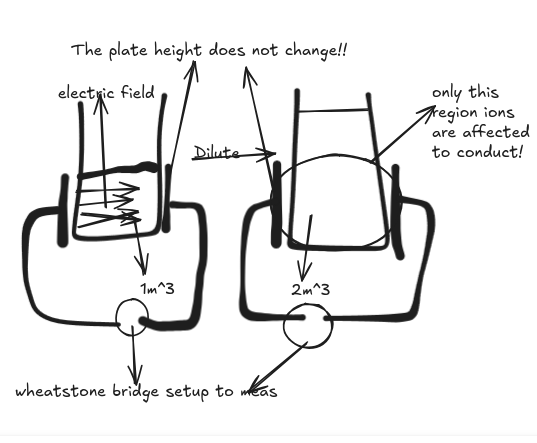
\includegraphics{Fig1.png}

\section*{Conductometric titration}
This is another way of doing titration without the use of indicator. We do this by keeping track of the ionic conductivity changes in the products of titration $\lambda_{ion}$ with respect to the analyte{we ignore the titrant because it is condumed as soon as it is added before we reach the eq. point}. This is done by measuring the ionic conductivity at various times in between, until we find the equivalence point.

The choice of the analyte can be of either weak or strong acid/base, the same goes for the titrant. Below are examples of systems like these and their behavior plotted.

\begin{figure}
\centering
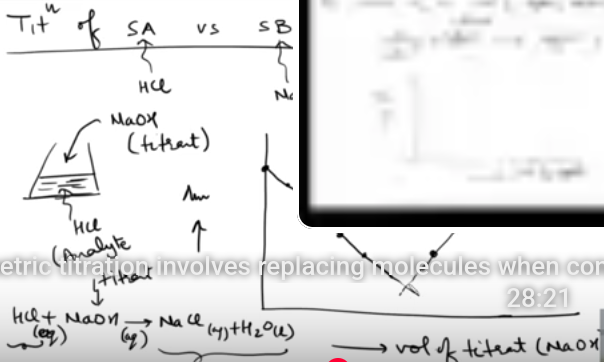
\includegraphics{Fig2.png}
\caption{A case of strong analyte and strong titrant}
\end{figure}

Here the titrant is NaOH and the analyte is HCl such that the H plus ions are consumed in the first half of this process and the OH minus ions poplulate in the second half.

\begin{figure}
\centering
\includegraphics{Fig3.png}
	\caption{A case of weak analyte and strong titrant}
\end{figure}

\clearpage
\begin{center}
{\Huge \textbf{SPACE LEFT FOR THIS LEC NOTES}}
\end{center}

\begin{itemize}

\item 

Why does a button cell stop providing its fixed value of potential difference abruptly rather than gradually like the dry cell}

This is because the reaction for the common mercury cell is $\ce{ZnHg + 2OH^{-} -> ZnO(s) + H_{2}O + 2e^{-}}$
for the anode and $\ce{HgO + H_{2}O + + 2e^{-} -> Hg(l) + 2OH^{-}}$, where the overall cell reaction then becomes.. $\ce{ZnHg + HgO -> ZnO(s) + Hg}$. This thing does not contain any reactant or porduct whose active mass may vary in the process of the cell function. Therefore from the nernst equation we can say that the potential here will be constant throughout the process.
